% ============================================================
% Plantilla de apuntes de Física
% Compilar con: pdflatex / latexmk -pdf
% ============================================================

\documentclass[12pt,oneside]{book}

% ------------------------------------------------------------
% PAQUETES
% ------------------------------------------------------------

% Idioma y codificación
\usepackage[utf8]{inputenc}
\usepackage[T1]{fontenc}
\usepackage[spanish,es-nodecimaldot]{babel}

% Márgenes
\usepackage[
    top=2.5cm,
    bottom=2.5cm,
    left=3cm,
    right=2.5cm,
    headheight=15pt
]{geometry}

% Matemática
\usepackage{amsmath}
\usepackage{amssymb}
\usepackage{mathtools}

% Física y unidades
\usepackage{siunitx}
\sisetup{
    output-decimal-marker = {,},
    per-mode = symbol,
    exponent-product = \cdot
}

% Imágenes y gráficos
\usepackage{graphicx}
\usepackage{float}
\usepackage{caption}
\usepackage{subcaption}

% Listas
\usepackage{enumitem}

% Colores y cajas
\usepackage{xcolor}
\usepackage[most]{tcolorbox}

% Tablas
\usepackage{booktabs}
\usepackage{array}

% Encabezados y pies
\usepackage{fancyhdr}

% Enlaces
\usepackage[
    colorlinks=true,
    linkcolor=blue!50!black,
    citecolor=green!40!black,
    urlcolor=blue!60!black,
    pdftitle={Apuntes de Física},
    pdfauthor={Isaac Edgar Camacho Ocampo},
    bookmarks=true
]{hyperref}

% ------------------------------------------------------------
% CONFIGURACIÓN GENERAL
% ------------------------------------------------------------

% Directorios donde buscar imágenes
\graphicspath{
    {./img/}
    {./graficos/}
    {./figuras/}
}

% Profundidad del índice
\setcounter{tocdepth}{2}

% Espaciado de párrafos
\setlength{\parindent}{0pt}
\setlength{\parskip}{0.5em}

% Listas
\setlist[itemize]{topsep=0.3em,itemsep=0.2em}
\setlist[enumerate]{topsep=0.3em,itemsep=0.2em}

% ------------------------------------------------------------
% ENCABEZADO Y PIE DE PÁGINA
% ------------------------------------------------------------

\pagestyle{fancy}
\fancyhf{}

\fancyhead[L]{\nouppercase{\leftmark}}
\fancyhead[R]{Física IA}

\fancyfoot[C]{\thepage}

\renewcommand{\headrulewidth}{0.4pt}
\renewcommand{\footrulewidth}{0pt}

% ------------------------------------------------------------
% COMANDOS MATEMÁTICOS
% ------------------------------------------------------------

% Vector
\newcommand{\vect}[1]{\mathbf{#1}}

% Derivadas
\newcommand{\deriv}[2]{\frac{d #1}{d #2}}
\newcommand{\derivn}[3]{\frac{d^{#3} #1}{d #2^{#3}}}

% Derivada parcial
\newcommand{\pderiv}[2]{\frac{\partial #1}{\partial #2}}

% Valor absoluto
\newcommand{\abs}[1]{\left|#1\right|}

% Norma
\newcommand{\norm}[1]{\left\lVert#1\right\rVert}

% ------------------------------------------------------------
% ENTORNOS PARA APUNTES
% ------------------------------------------------------------

% Definición
\newtcolorbox{definition}[1]{
    enhanced,
    breakable,
    title={Definición: #1},
    fonttitle=\bfseries,
    colback=blue!3,
    colframe=blue!50!black,
    boxrule=0.8pt,
    arc=2mm
}

% Concepto importante
\newtcolorbox{important}{
    enhanced,
    breakable,
    title={Importante},
    fonttitle=\bfseries,
    colback=yellow!8,
    colframe=orange!70!black,
    boxrule=0.8pt,
    arc=2mm
}

% Ejemplo
\newtcolorbox{example}[1]{
    enhanced,
    breakable,
    title={Ejemplo: #1},
    fonttitle=\bfseries,
    colback=green!4,
    colframe=green!40!black,
    boxrule=0.8pt,
    arc=2mm
}

% Fórmula importante
\newtcolorbox{formula}[1]{
    enhanced,
    breakable,
    title={Fórmula: #1},
    fonttitle=\bfseries,
    colback=purple!4,
    colframe=purple!50!black,
    boxrule=0.8pt,
    arc=2mm
}

% Ejercicio
\newtcolorbox{exercise}[1]{
    enhanced,
    breakable,
    title={Ejercicio: #1},
    fonttitle=\bfseries,
    colback=gray!5,
    colframe=gray!60!black,
    boxrule=0.8pt,
    arc=2mm
}

% ------------------------------------------------------------
% DOCUMENTO
% ------------------------------------------------------------

\begin{document}

% ============================================================
% PORTADA
% ============================================================

\begin{titlepage}

\thispagestyle{empty}

\begin{center}

\vspace*{1cm}

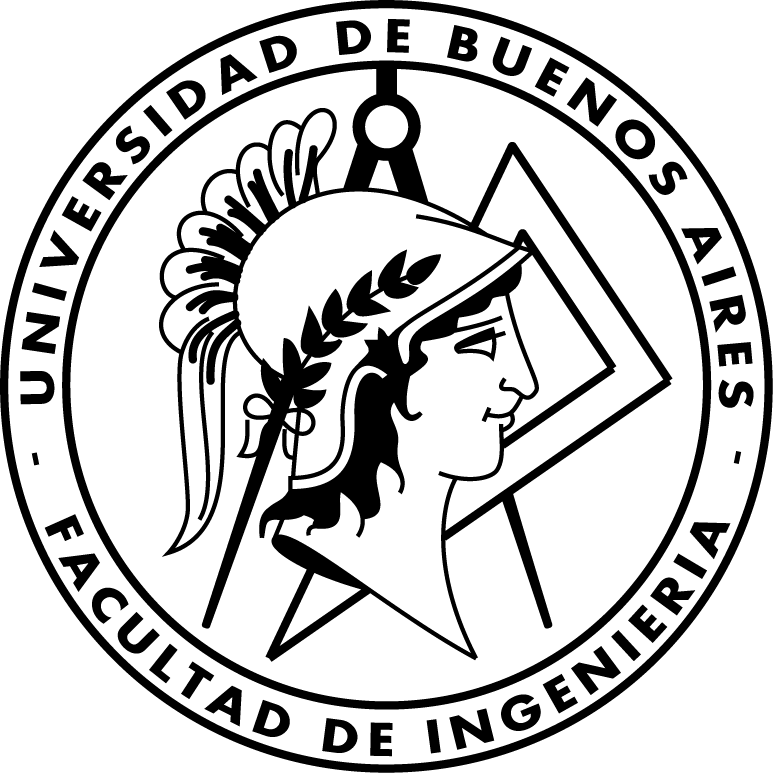
\includegraphics[width=0.35\textwidth]{Logo-fiuba_big.png}

\vspace{1.5cm}

{\large UNIVERSIDAD DE BUENOS AIRES}

\vspace{0.2cm}

{\large FACULTAD DE INGENIERÍA}

\vspace{2.5cm}

{\Huge \textbf{FÍSICA IA}}

\vspace{0.7cm}

{\Large Apuntes de Física}

\vspace{1.5cm}

\rule{0.7\textwidth}{0.5pt}

\vspace{0.5cm}

{\large Mecánica y fundamentos de Física}

\vspace{0.5cm}

\rule{0.7\textwidth}{0.5pt}

\vfill

{\large Isaac Edgar Camacho Ocampo}

\vspace{0.3cm}

{\large Buenos Aires}

{\large \the\year}

\end{center}

\end{titlepage}

% ============================================================
% ÍNDICE
% ============================================================

\tableofcontents

\clearpage

% ============================================================
% CAPÍTULO 1
% ============================================================

\chapter{Cinemática}

La cinemática es la rama de la mecánica que estudia el
movimiento de los cuerpos sin analizar las causas que lo
producen.

\section{Conceptos fundamentales}

\begin{definition}{Partícula}
Una partícula es un modelo físico en el que se considera que
las dimensiones del cuerpo son despreciables frente a las
distancias involucradas en el problema.
\end{definition}

\begin{definition}{Sistema de referencia}
Un sistema de referencia es un conjunto de coordenadas y una
referencia temporal que permite describir la posición y el
movimiento de un cuerpo.
\end{definition}

\section{Posición y desplazamiento}

La posición de una partícula puede representarse mediante un
vector:

\begin{equation}
    \vect{r}(t) = x(t)\,\hat{\imath}
    + y(t)\,\hat{\jmath}
    + z(t)\,\hat{k}.
    \label{eq:posicion}
\end{equation}

El desplazamiento entre dos instantes se define como:

\begin{equation}
    \Delta \vect{r}
    = \vect{r}_f - \vect{r}_i.
    \label{eq:desplazamiento}
\end{equation}

\begin{important}
El desplazamiento es una magnitud vectorial. La distancia
recorrida, en cambio, es una magnitud escalar.
\end{important}

\section{Velocidad}

La velocidad media se define como:

\begin{equation}
    \vect{v}_{\text{med}}
    =
    \frac{\Delta \vect{r}}{\Delta t}.
    \label{eq:velocidad-media}
\end{equation}

La velocidad instantánea es:

\begin{equation}
    \vect{v}(t)
    =
    \deriv{\vect{r}}{t}.
    \label{eq:velocidad}
\end{equation}

\begin{formula}{Velocidad instantánea}
\[
    \boxed{
    \vect{v}(t)=\frac{d\vect{r}}{dt}
    }
\]
\end{formula}

\section{Aceleración}

La aceleración mide la variación temporal de la velocidad:

\begin{equation}
    \vect{a}(t)
    =
    \deriv{\vect{v}}{t}
    =
    \derivn{\vect{r}}{t}{2}.
    \label{eq:aceleracion}
\end{equation}

\begin{example}{Movimiento uniformemente acelerado}
Si la aceleración es constante,

\[
    \vect{a} = \text{constante},
\]

entonces la velocidad y la posición pueden obtenerse mediante:

\[
    \vect{v}(t)
    =
    \vect{v}_0 + \vect{a}t
\]

y

\[
    \vect{r}(t)
    =
    \vect{r}_0
    + \vect{v}_0 t
    + \frac{1}{2}\vect{a}t^2.
\]
\end{example}

% Ejemplo de imagen:
%
% \begin{figure}[H]
%     \centering
%     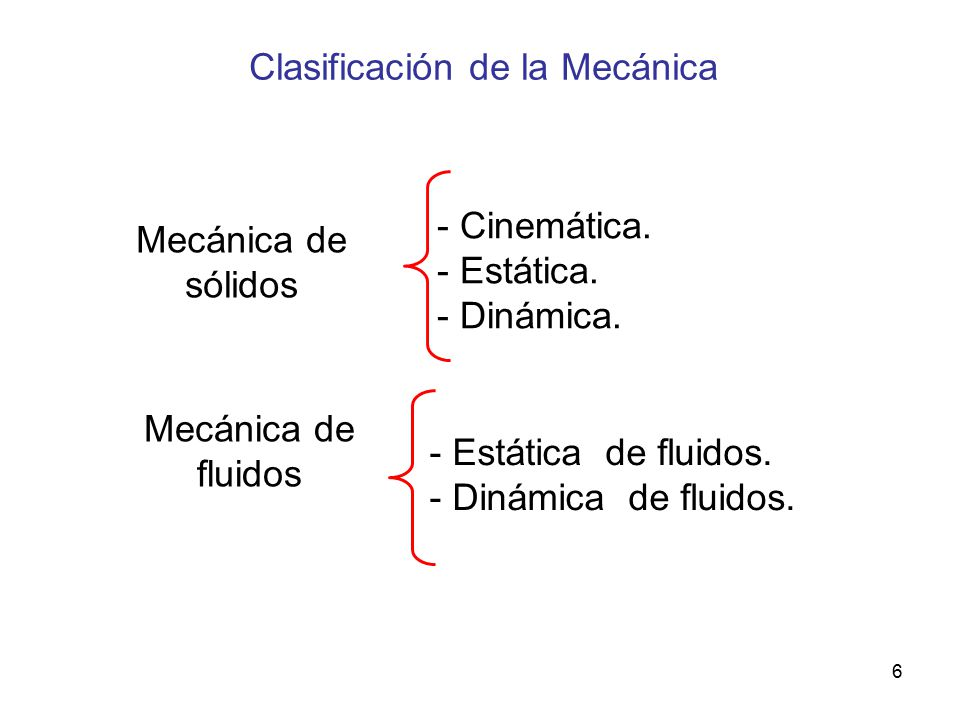
\includegraphics[width=0.8\textwidth]{01}
%     \caption{Ejemplo de movimiento.}
%     \label{fig:movimiento}
% \end{figure}

% ============================================================
% CAPÍTULO 2
% ============================================================

\chapter{Dinámica}

La dinámica estudia la relación entre el movimiento de los
cuerpos y las fuerzas que actúan sobre ellos.

\section{Fuerza}

\begin{definition}{Fuerza}
Una fuerza es una interacción capaz de modificar el estado de
movimiento de un cuerpo o producir una deformación.
\end{definition}

\section{Leyes de Newton}

\subsection{Primera ley de Newton}

\begin{important}
Si la fuerza neta sobre un cuerpo es cero, el cuerpo mantiene
su estado de reposo o de movimiento rectilíneo uniforme.
\end{important}

\subsection{Segunda ley de Newton}

\begin{formula}{Segunda ley de Newton}
\[
    \boxed{
    \sum \vect{F} = m\vect{a}
    }
\]
\end{formula}

\subsection{Tercera ley de Newton}

Para toda fuerza ejercida por un cuerpo sobre otro existe una
fuerza de igual magnitud y dirección opuesta ejercida por el
segundo cuerpo sobre el primero.

% ============================================================
% CAPÍTULO 3
% ============================================================

\chapter{Trabajo y energía}

\section{Trabajo}

\section{Energía cinética}

\section{Energía potencial}

\section{Conservación de la energía}

% ============================================================
% CAPÍTULO 4
% ============================================================

\chapter{Cantidad de movimiento}

\section{Momento lineal}

\section{Impulso}

\section{Conservación del momento lineal}

% ============================================================
% CAPÍTULO 5
% ============================================================

\chapter{Oscilaciones}

\section{Movimiento armónico simple}

\section{Péndulo simple}

% ============================================================
% APÉNDICES
% ============================================================

\appendix

\chapter{Fórmulas y constantes}

\section{Constantes físicas}

Por ejemplo:

\[
    g \approx \SI{9.81}{\meter\per\second\squared}
\]

\section{Conversión de unidades}

% ============================================================
% BIBLIOGRAFÍA
% ============================================================

\begin{thebibliography}{9}

\bibitem{serway}
Raymond A. Serway y John W. Jewett,
\textit{Física para ciencias e ingeniería}.

\bibitem{halliday}
David Halliday, Robert Resnick y Jearl Walker,
\textit{Fundamentos de Física}.

\end{thebibliography}

\end{document}
